\chapter{Requisitos Funcionais}

\section{Âmbito do projecto}

\subsection{Situação actual}

Actualmente, o mercado financeiro de retalho oferece aos seus clientes uma grande variedade de simuladores de produtos de seguros, como os do ramo automóvel, motociclo, ciclomotor, saúde, habitação, etc. Aparte a simulação efectuada presencialmente com um Mediador, as várias Seguradoras oferecem uma interface \emph{Web} para a simulação dos seus produtos. No entanto, apenas conferem a opção de simular individualmente cada um dos produtos, não permitindo que seja efectuada uma simulação agregada de vários produtos oferecidos pela mesma Seguradora, com a possibilidade de se auferirem descontos em função de diversos factores como o perfil do utilizador, quantidade de produtos a contratar e o valor do prémio acumulado. Suprir esta lacuna é o mote para o desenvolvimento deste sistema de informação que deverá, paralelamente, permitir a configuração, validação e produção de simuladores para produtos financeiros.

\subsection{Contexto do projecto}

De forma a integrar melhor o sistema a desenvolver nas actividades quotidianas, é imperativo que se modele um diagrama de contexto, que clarifique quais as entidades externas ao sistema informático que vão ter algum relacionamento com este, isto é, quais as actividades que o sistema informático vai suportar no negócio em questão. Desta forma foram elaborados vários diagramas de contexto que visam clarificar essas actividades:

\begin{itemize}

\item \textbf{Diagrama de Contexto de Alto Nível}, onde apenas se apresentam o sistema e os actores que com ele vão interagir:

\begin{figure}[!htb]
	\centering
	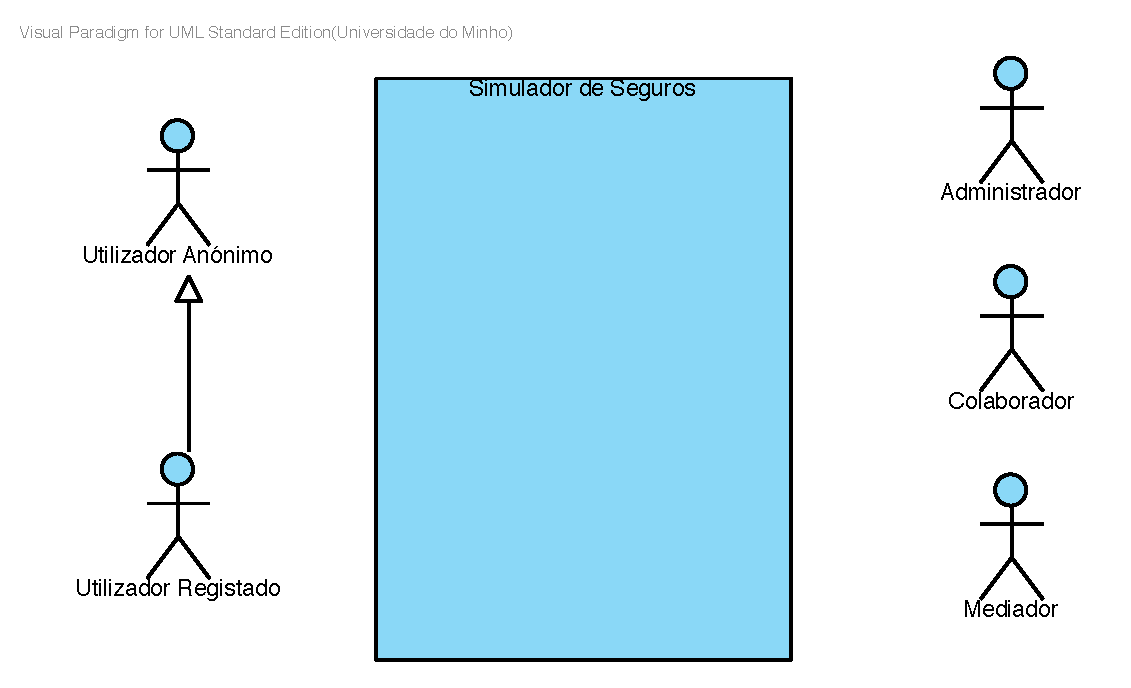
\includegraphics[scale=0.8]{images/DiagramaContextoAltoNivel}
	\caption{Diagrama de Contexto de Alto Nível}
\end{figure}

\item \textbf{Diagrama de Contexto de cada um dos actores}, onde se apresentam as acções realizáveis por cada actor no sistema (Administrador, Colaborador, Mediador, Utilizador Registado e Utilizador Anónimo):

\begin{figure}[!htb]
	\centering
	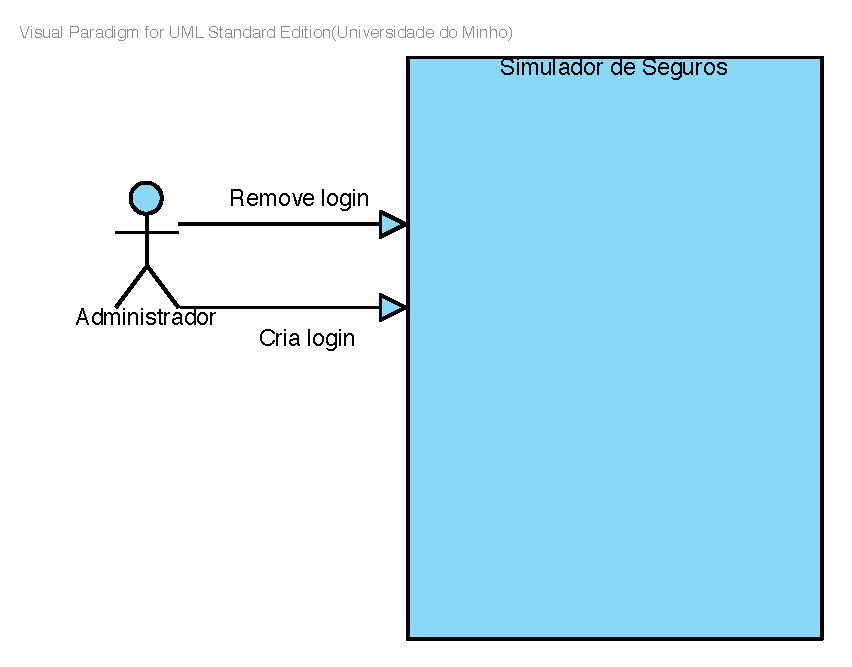
\includegraphics[scale=0.75]{images/DiagramaContextoAdministrador}
	\caption{Diagrama de Contexto do Administrador}
\end{figure}

\begin{figure}[!htb]
	\centering
	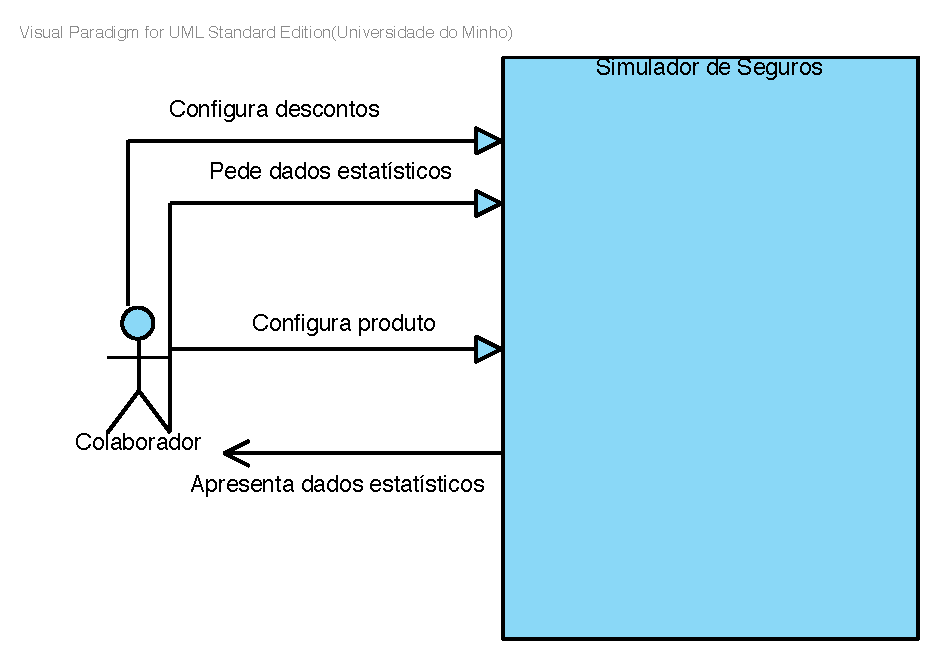
\includegraphics[scale=0.75]{images/DiagramaContextoColaborador}
	\caption{Diagrama de Contexto do Colaborador}
\end{figure}

\begin{figure}[!htb]
	\centering
	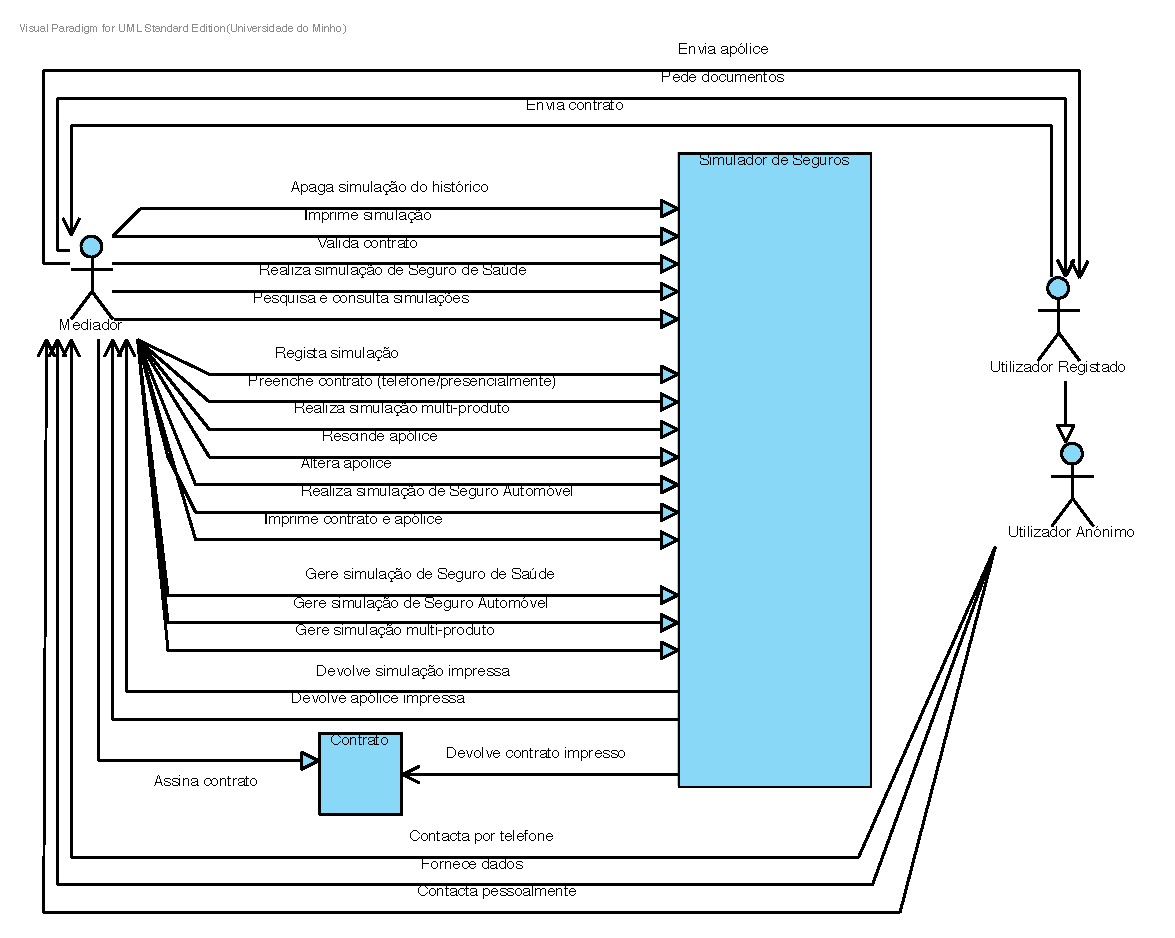
\includegraphics[scale=0.9]{images/DiagramaContextoMediador}
	\caption{Diagrama de Contexto do Mediador}
\end{figure}

\begin{figure}[!htb]
	\centering
	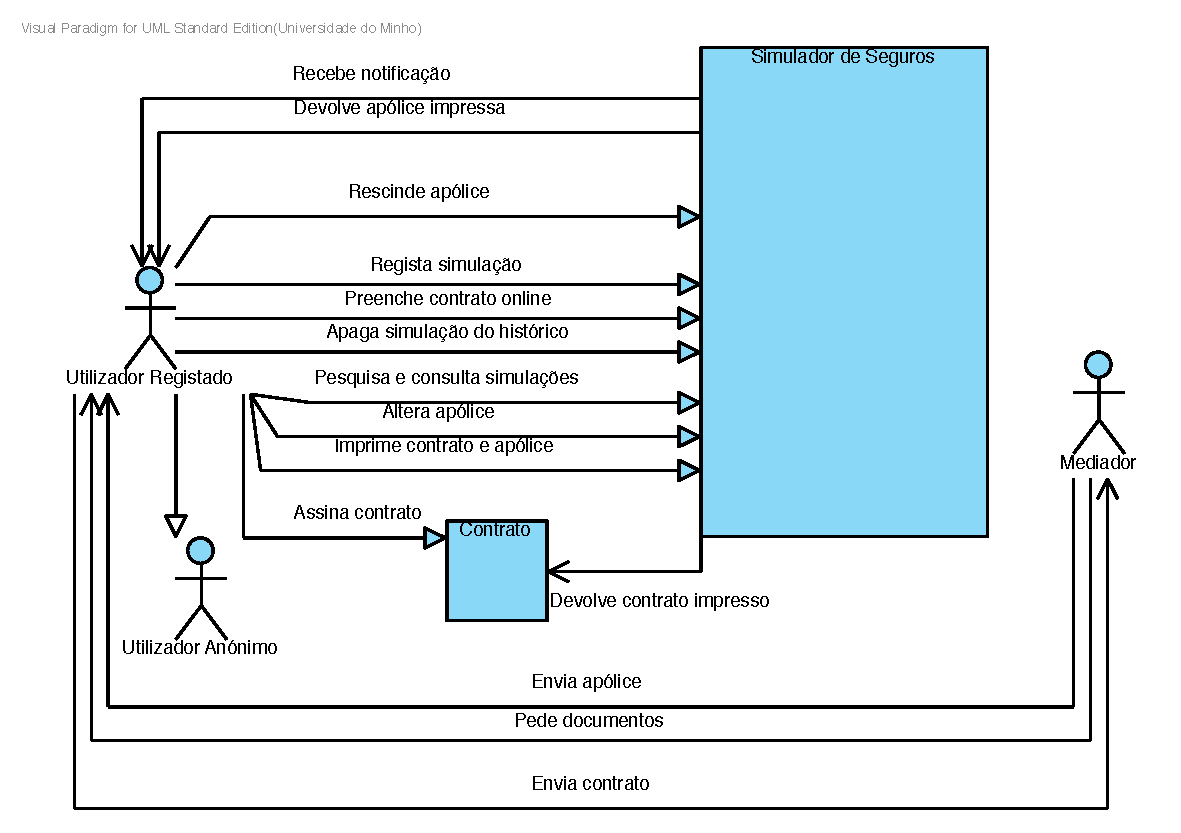
\includegraphics[scale=0.7]{images/DiagramaContextoUtilizadorRegistado}
	\caption{Diagrama de Contexto do Utilizador Registado}
\end{figure}

\begin{figure}[!htb]
	\centering
	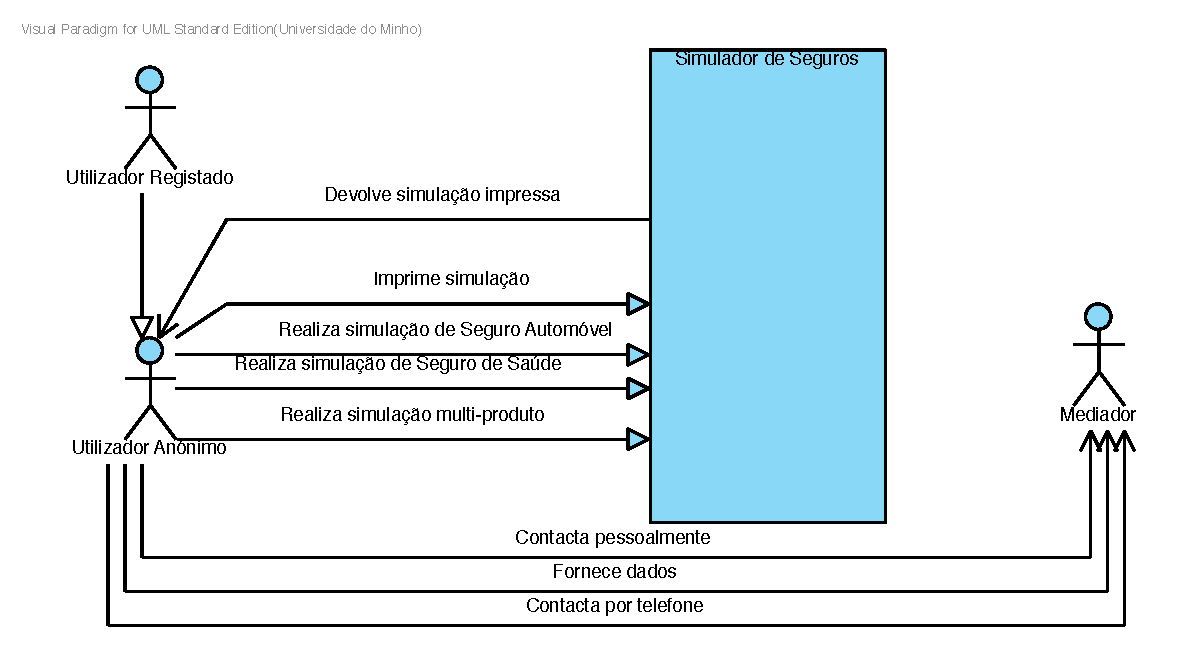
\includegraphics[scale=0.7]{images/DiagramaContextoUtilizadorAnonimo}
	\caption{Diagrama de Contexto do Utilizador Anónimo}
\end{figure}
\pagebreak 
\subsubsection*{ }
\pagebreak
\subsubsection*{ }
\pagebreak


\item \textbf{Diagrama de Contexto de Baixo Nível}, que agrega os diagramas dos vários actores:

\begin{figure}[!htb]
	\centering
	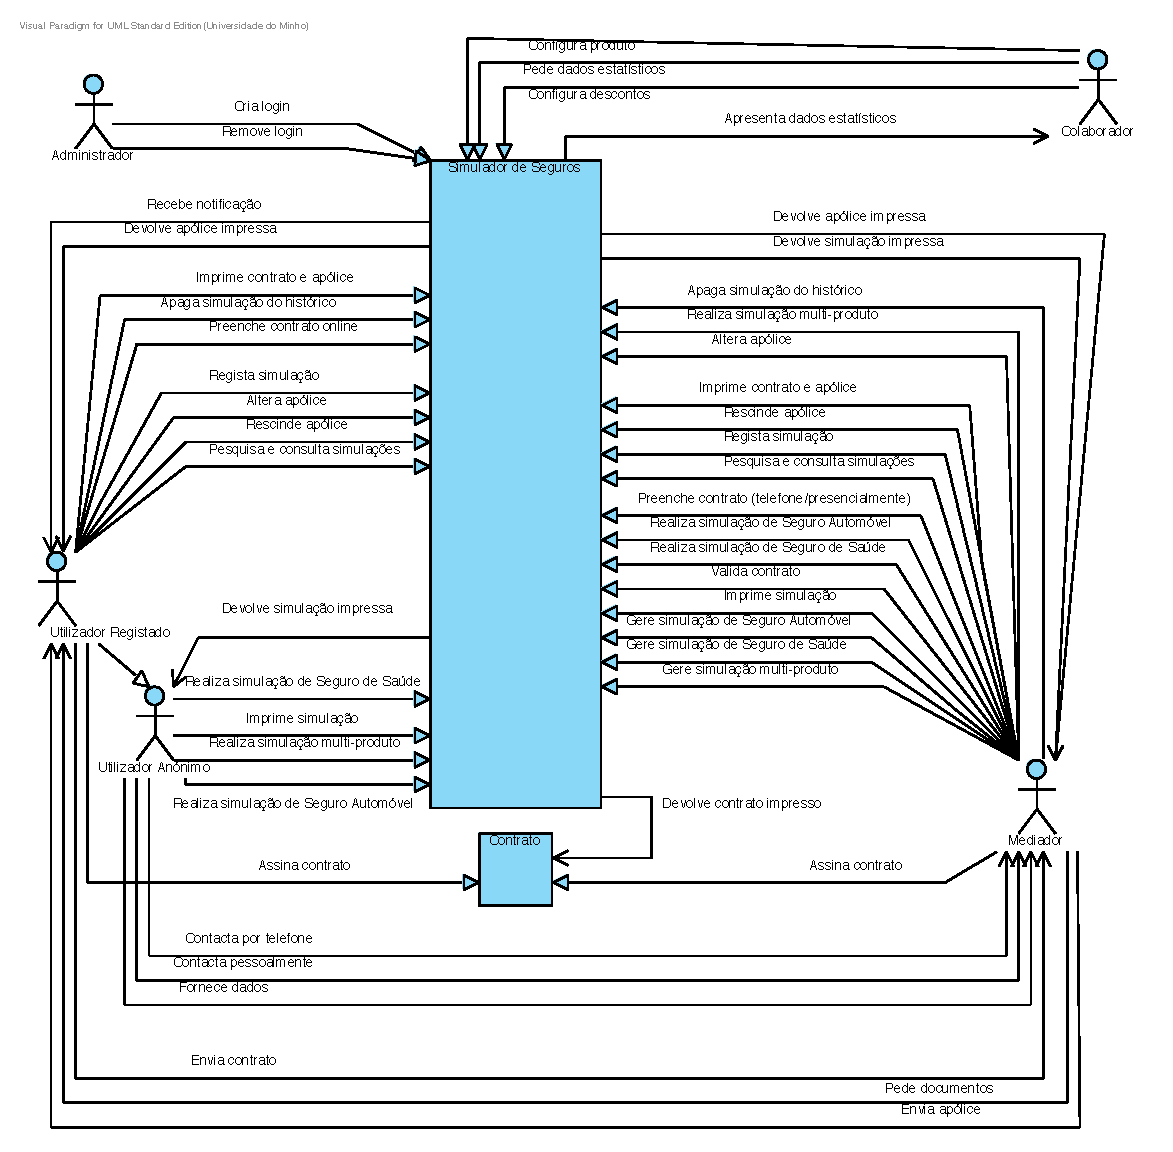
\includegraphics[scale=0.9]{images/DiagramaContextoBaixoNivel}
	\caption{Diagrama de Contexto de Baixo Nível}
\end{figure}

\end{itemize}

\subsection{Divisão do projecto}

Para responder aos eventos do negócio, criam-se os \emph{Business Use Cases} que modelam um determinado evento de negócio que ocorre entre um actor e o sistema, indicando-se o nome do evento, os dados provenientes de outros sistemas e os resultados obtidos no final. Estes \emph{Use Cases} permitem descobrir os vários subsistemas do sistema principal que promovem a interacção entre utilizador e sistema. Listam-se de seguida aqueles que foram definidos para o sistema em questão:

\pagebreak
\begin{table}[!htb]
	\begin{center}
		\begin{tabular}{|c|p{3cm}|p{3cm}|p{5cm}|}
		\hline
		\multicolumn{1}{|c|}{\textbf{Número}} & \multicolumn{1}{|c|}{\textbf{Nome do Evento}} & \multicolumn{1}{|c|}{\textbf{Input / Output}} & \multicolumn{1}{|c|}{\textbf{Breve descrição}}\\
		\hline
		\T \B 1 & \scriptsize{Realizar simulação de Seguro Automóvel} & \scriptsize{Simulação realizada e é apresentado o nome do produto e valores a pagar. (out)} & \scriptsize{Utilizador (Anónimo / Registado) / Mediador realiza uma simulação para o seu Seguro Automóvel, tendo em conta os dados introduzidos pelo Utilizador (Anónimo / Registado) / Mediador.}\\
		\hline
		\T \B 2 & \scriptsize{Realizar simulação de Seguro de Saúde} & \scriptsize{Simulação realizada e é apresentado o nome do produto e valores a pagar. (out)} & \scriptsize{Utilizador (Anónimo / Registado) / Mediador realiza uma simulação para o seu Seguro de Saúde, tendo em conta os dados introduzidos pelo Utilizador (Anónimo / Registado) / Mediador.}\\
		\hline
		\T \B 3 & \scriptsize{Realizar simulação multi-produto} & \scriptsize{Simulação realizada e é apresentado os nomes dos produtos e valores a pagar. (out)} & \scriptsize{Utilizador (Anónimo / Registado) / Mediador realiza uma simulação agregada de vários produtos de seguros, tendo em conta os dados introduzidos pelo Utilizador (Anónimo / Registado) / Mediador.}\\
		\hline
		\T \B 4 & \scriptsize{Pesquisar e consultar simulações} & \scriptsize{Conjunto de simulações efectuadas é apresentado e são apresentados os dados da simulação consultada. (out)} & \scriptsize{Utilizador (Registado) / Mediador realiza uma pesquisa das simulações por si efectuadas (Mediador pode pesquisar também as dos seus clientes) e consulta a simulação desejada.}\\
		\hline
		\T \B 5 & \scriptsize{Rescindir Apólice} & \scriptsize{Sistema confere o carácter nulo ao contrato. (out)} & \scriptsize{Utilizador (Registado) / Mediador solicita a rescisão do contrato previamente estabelecido.}\\
		\hline
		\T \B 6 & \scriptsize{Alterar Apólice} & \scriptsize{Sistema altera dados presentes no contrato. (out)} & \scriptsize{Utilizador (Registado) / Mediador solicita alteração dos dados presentes no contrato.}\\
		\hline
		\T \B 7 & \scriptsize{Pedir dados estatísticos} & \scriptsize{Sistema apresenta dados recolhidos para estatística. (out)} & \scriptsize{Colaborador solicita a visualização dos dados estatísticos referentes às simulações efectuadas.}\\
		\hline
		\T \B 8 & \scriptsize{Configurar descontos} & \scriptsize{Alteração dos descontos existentes. (out)} & \scriptsize{Colaborador altera os parâmetros utilizados no cálculo dos descontos a aplicar.}\\
		\hline
		\T \B 9 & \scriptsize{Registar simulação} & \scriptsize{Sistema regista simulação e actualiza dados estatísticos. (out)} & \scriptsize{Utilizador (Registado) / Mediador regista simulação efectuada no sistema.}\\
		\hline
		\T \B 10 & \scriptsize{Apagar simulação do histórico} & \scriptsize{Sistema apaga simulação e dados estatísticos actualizados. (out)} & \scriptsize{Utilizador (Registado) / Mediador apaga do seu histórico simulações por si efectuadas (Mediador apagas as simulações feitas por si e pelos seus clientes).}\\
		\hline
		\end{tabular}
		\caption{\emph{Business Use Cases} (1$\to$10)}
	\end{center}
\end{table}

\pagebreak
\begin{table}[!htb]
	\begin{center}
		\begin{tabular}{|c|p{3cm}|p{3cm}|p{5cm}|}
		\hline
		\multicolumn{1}{|c|}{\textbf{Número}} & \multicolumn{1}{|c|}{\textbf{Nome do Evento}} & \multicolumn{1}{|c|}{\textbf{Input / Output}} & \multicolumn{1}{|c|}{\textbf{Breve descrição}}\\
		\hline
		\T \B 11 & \footnotesize{Contactar por telefone} & \footnotesize{Solicitação de simulação. (out)} & \footnotesize{Utilizador (Anónimo / Registado) contacta Mediador por telefone com vista a efectuar simulação.}\\
		\hline
		\T \B 12 & \footnotesize{Contactar pessoalmente} & \footnotesize{Solicitação de simulação. (out)} & \footnotesize{Utilizador (Anónimo / Registado) contacta Mediador pessoalmente com vista a efectuar simulação.}\\
		\hline
		\T \B 13 & \footnotesize{Fornecer dados} & \footnotesize{Mediador recebe dados fornecidos. (out)} & \footnotesize{Utilizador (Anónimo / Registado) fornece ao Mediador os dados necessários à realização de uma simulação. ("<extends"> Contactar por telefone / Contactar pessoalmente).}\\
		\hline
		\T \B 14 & \footnotesize{Pedir documentos} & \footnotesize{Fotocópias dos documentos solicitados. (out)} & \footnotesize{Mediador solicita ao Utilizador (Registado) que lhe forneça os documentos necessários à contratação, para fotocópia.}\\
		\hline
		\T \B 15 & \footnotesize{Preencher contrato online} & \footnotesize{Contrato de seguro preenchido. (out)} & \footnotesize{Utilizador (Registado) preenche o contrato de seguro.}\\
		\hline
		\T \B 16 & \footnotesize{Preencher contrato (telefone / presencialmente)} & \footnotesize{Contrato de seguro preenchido. (out)} & \footnotesize{Mediador preenche o contrato de seguro para o Utilizador(Registado).}\\
		\hline
		\T \B 17 & \footnotesize{Imprimir contrato e apólice} & \footnotesize{Contrato e apólice impressos. (out)} & \footnotesize{Utilizador (Registado) / Mediador solicita a impressão do contrato e apólice.}\\
		\hline
		\T \B 18 & \footnotesize{Assinar contrato} & \footnotesize{Contrato assinado. (out)} & \footnotesize{Utilizador (Registado) / Mediador assina contrato de seguro.}\\
		\hline
		\T \B 19 & \footnotesize{Validar contrato} & \footnotesize{Contrato validado. (out)} & \footnotesize{Mediador consulta o contrato estabelecido e valida-o.}\\
		\hline
		\T \B 20 & \footnotesize{Imprimir simulação} & \footnotesize{Simulação impressa. (out)} & \footnotesize{Utilizador (Anónimo / Registado) / Mediador solicita a impressão de simulação.}\\
		\hline
		\end{tabular}
		\caption{\emph{Business Use Cases} (11$\to$20)}
	\end{center}
\end{table}
\pagebreak

\begin{table}[!htb]
	\begin{center}
		\begin{tabular}{|c|p{3cm}|p{3cm}|p{5cm}|}
		\hline
		\textbf{Número} & \textbf{Nome do Evento} & \textbf{Input / Output} & \textbf{Breve descrição}\\
		\hline
		\T \B 21 & \footnotesize{Gerir Simulação de Seguro Automóvel} & \footnotesize{Simulação efectuada e notificação possivelmente enviada. (out)} & \footnotesize{Mediador, após ser contactado pelo Utilizador, selecciona-o da lista de clientes a si afectos e inicia a sua simulação, e no fim envia, possivelmente, uma notificação para a área do Utilizador (Registado).}\\
		\hline
		\T \B 22 & \footnotesize{Gerir Simulação de Seguro de Saúde} & \footnotesize{Simulação efectuada e notificação possivelmente enviada. (out)} & \footnotesize{Mediador, após ser contactado pelo Utilizador, selecciona-o da lista de clientes a si afectos e inicia a sua simulação, e no fim envia, possivelmente, uma notificação para a área do Utilizador (Registado).}\\
		\hline
		\T \B 23 & \footnotesize{Gerir Simulação multi-produto} & \footnotesize{Simulação efectuada e notificação possivelmente enviada. (out)} & \footnotesize{Mediador, após ser contactado pelo Utilizador, selecciona-o da lista de clientes a si afectos e inicia a sua simulação, e no fim envia, possivelmente, uma notificação para a área do Utilizador (Registado).}\\
		\hline
		\T \B 24 & \footnotesize{Configurar produto} & \footnotesize{Produto do sistema adicionado / removido / alterado. (out)} & \footnotesize{Colaborador adiciona, remove ou edita produto.}\\
		\hline
		\T \B 25 & \footnotesize{Criar login} & \footnotesize{Login criado. (out)} & \footnotesize{Administrador cria login para determinado Mediador ou Colaborador.}\\
		\hline
		\T \B 26 & \footnotesize{Remover login} & \footnotesize{Login removido. (out)} & \footnotesize{Administrador remove do sistema um login anteriormente criado por um Mediador ou Colaborador.}\\
		\hline
		\T \B 27 & \footnotesize{Enviar contrato} & \footnotesize{Contrato enviado. (out)} & \footnotesize{Utilizador (Registado) envia contrato para o Mediador.}\\
		\hline
		\T \B 28 & \footnotesize{Enviar apólice} & \footnotesize{Apólice enviada. (out)} & \footnotesize{Mediador envia apólice para o Utilizador (Registado).}\\
		\hline
		\end{tabular}
		\caption{\emph{Business Use Cases} (21$\to$28)}
	\end{center}
\end{table}
\pagebreak
Com isto, já há material suficiente para conseguir definir os seguintes subsistemas:

\begin{itemize}
\item Simulador Automóvel
\item Simulador Saúde
\item Simulação Multi-Produto
\item Pesquisa e consulta de simulações
\item Contratação
\item Estatísticas de utilização do sistema
\item Configuração de descontos
\item Registo de simulações
\item Impressão de documentos
\end{itemize}